\documentclass{standalone}

% Plotting
\usepackage{tikz}
\usetikzlibrary{decorations.markings}
\usetikzlibrary{calc}
% quantikz breaks tikz-cd, see https://tex.stackexchange.com/questions/618330/quantikz-breaks-spacing-in-tikz-matrices-tikz-cd
%\usetikzlibrary{quantikz}
\usetikzlibrary{cd}
\usepackage{pgfplots}

\usepackage{simpler-wick}
\usepackage{physics}

\usepackage{amsmath}
\usepackage{mathtools}

\begin{document}
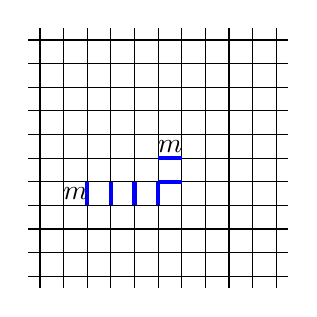
\begin{tikzpicture}[scale=1.5, decoration={
    markings,
    mark=at position 0.5 with {\arrow{>}}}]

    \foreach \i in {0,0.2,...,2} {
        \draw (\i, -0.1) -- (\i, 2.1);
    }

    \foreach \i in {0,0.2,...,2} {
        \draw (-0.1, \i) -- (2.1, \i);
    }

    \draw[ultra thick, blue] (0.4, 0.6) -- ++(0, 0.2);
    \draw[ultra thick, blue] (0.6, 0.6) -- ++(0, 0.2);
    \draw[ultra thick, blue] (0.8, 0.6) -- ++(0, 0.2);
    \draw[ultra thick, blue] (1, 0.6) -- ++(0, 0.2);
    \draw[ultra thick, blue] (1, 0.8) -- ++(0.2, 0);
    \draw[ultra thick, blue] (1, 1) -- ++(0.2, 0);

    \draw (0.3, 0.7) node {$m$};
    \draw (1.1, 1.1) node {$m$};
\end{tikzpicture}
\end{document}